\section{Introduction}\label{sec:intro}

In the present day, the efficient computation of large-scale data has become a necessity. 
In particular, various areas such as biological networks, social networks,
financial markets, energy grids, etc. give rise to large-scale graph data. In
order to develop faster algorithms to process large-scale data (especially graph
data), several large-scale graph processing systems such as Pregel~\cite{pregel},
Giraph~\cite{Giraph}, and Spark's GraphX~\cite{graphx} have been designed based
on the \emph{message-passing} distributed computing model~\cite{Lynch96,Peleg00}.
In these systems, the input graph, which is simply too large to fit into a single
machine, is distributed across a group of machines that are connected via a
communication network and the machines jointly perform computation in a
distributed fashion by sending/receiving messages.

The focus of this paper is the \(k\)-machine model, introduced
in~\cite{KlauckNPR15}, which  is a message-passing distributed computing model
for large-scale computations (see \cref{sec:model}). Several papers have
developed algorithms in this model for various graph problems~\cite{KlauckNPR15,topc18,BandyapadhyayIPP18,PRS21,pemmaraju-opodis18,peter,gilbert,ipdps21}.
The \(k\)-machine model is a distributed \emph{complete} network of \(k\)
machines (nodes) that communicate through message passing over
\emph{bandwidth-restricted} links. The input is some set of data, usually a
graph, distributed across the machines, typically in a balanced fashion. The
machines are synchronous, i.e., they proceed in a sequence of rounds, wherein
each machine performs some local computation and can send and receive messages.
The goal is to minimize the \emph{round complexity}, i.e., the number of
communication rounds; in particular, to obtain bounds that scale well with $k$.
Hence, algorithms proposed for the \(k\)-machine model are evaluated solely on
the basis of their round complexity. The motivation behind this is that in
large-scale distributed data processing, communication is significantly more
time-consuming than local computation \cite{KlauckNPR15,topc18,cacm}.
Thus, analysis in this model assumes local computation (within a machine)
is  ``free.''

The above assumption, that we can simply ignore local computation cost and focus
only on the communication cost, can be a good approximation to the overall time
complexity where computation cost of individual machines is significantly smaller
than communication cost. This could be true when processor speeds are
significantly faster than network speeds and for very large-scale data
communication. However, modern networks have become much faster, resulting in
the need to evaluate algorithms in a more nuanced manner. As network speeds
approach that of processor speeds, it is not necessarily the case that the
bottleneck for computation lies only in how many communication rounds of message
passing are required. Moreover, for moderately-sized data, the communication
cost may not be significantly higher than the computation cost. This all means
that, in general, computation cost should also be taken into account. This is
typically seen in practical implementations of \(k\)-machine model algorithms,
where wall-clock time speed up is upper bounded by \(\sfrac{1}{k}\), i.e., one
cannot expect to see more than a linear speed up.  To give an example, we
implemented an efficient, distributed $k$-machine algorithm (using MPI) for
computing PageRank from~\cite{KlauckNPR15}. This algorithm has a round
complexity of \(\bigO{\sfrac{n}{k}}\). \Cref{fig:pr} shows how the execution
time (wall clock time) scales with respect to the number of machines. The
scaling is proportional to (approximately) \(\bigO{\sfrac{1}{k^{0.8}}}\) and is
less than the linear scaling (i.e., \(\bigO{\sfrac{1}{k}}\)) predicted by the
analysis. We also implemented a more sophisticated algorithm for PageRank from
\cite{PRS21} that has round complexity \(\bigO{n/k^2}\) (which is optimal up to
polylogarithmic factors). Note that this round complexity scales super-linearly
(i.e., quadratically) with the number of machines. However, the execution time
of this algorithm also has less than linear scaling, since local computation
still has a significant cost. 

Hence it is necessary to augment the \(k\)-machine model with a means to capture
the local computation performed on each machine. In this paper, we propose such
an augmented \(k\)-machine model where, in addition to the communication round
complexity that is traditionally measured, we also measure the local computation
performed by the machines over all rounds. We utilize this framework to analyze
solutions to two fundamental graph problems, connectivity (more generally,
finding connected components) and minimum spanning tree (MST) of undirected
graphs. Connected components can be used as a fundamental subroutine in several
other graph algorithms, such as testing $st$-connectivity, bipartiteness
checking, approximate min-cut, and several graph verification problems (see
e.g. \cite{topc18}) and graph clustering (see e.g. \cite{KiverisLMRV14}),
which in turn are fundamental tools that can be applied to solve practical problems
in machine learning, social network analysis, pattern recognition, and
information retrieval. The MST is useful for a variety of tasks including
information dissemination and has been studied in various models due to its
importance (see e.g. \cite{KlauckNPR15,AGGHSKL19,GallagerHS83}).

\begin{figure}[t]
    \centering
    \scriptsize
    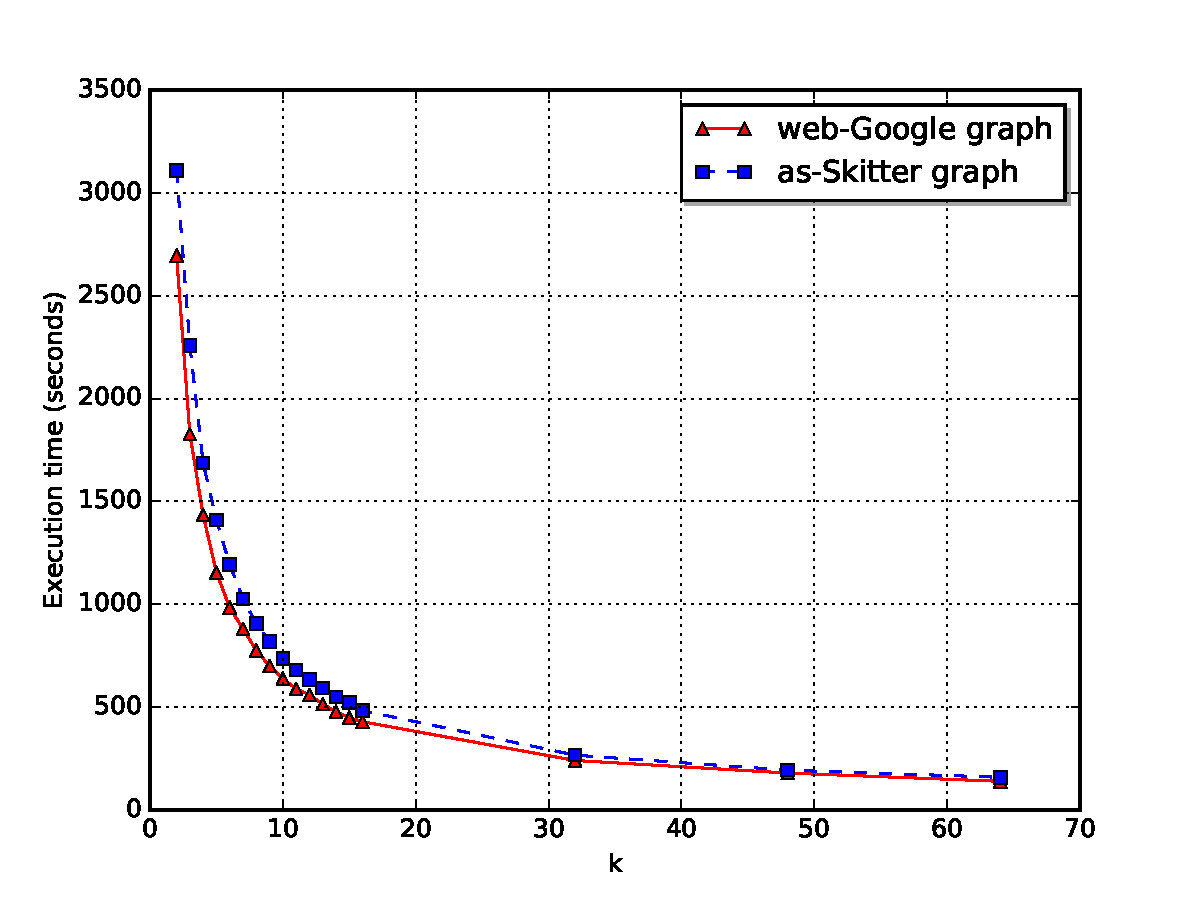
\includegraphics[height=2in,width=2in]{diag}
    \vspace{-0.25in}
    \caption{\scriptsize Performance of the distributed PageRank Algorithm of
	\cite{KlauckNPR15} on two graphs from Stanford Network Analysis Project
	(\url{snap.stanford.edu}): Google Web graph (875713 nodes) and Autonomous
	System by Skitter (1.69M nodes). The algorithm was implemented using MPI and
	run on a cluster of machines interconnected by a high speed network. The
	graph shows that the execution time is proportional (approximately) to
	$\sfrac{1}{k^{0.8}}$.}\label{fig:pr}
\end{figure}

\subsection{Model and Complexity measures}\label{sec:model}
We generalize the \emph{\(k\)-machine} model by incorporating an additional
metric to evaluate the efficiency of algorithms. We first introduce the basic
model (e.g. \cite{KlauckNPR15}) and subsequently introduce our metric.

The standard \(k\)-machine model has \(k\) machines \(M_1, M_2, \hdots, M_k\)
connected together in a clique using bidirectional communication links. The
machines operate in synchronous rounds. The input to this system is a graph
\(G = (V,E)\) with \(|V| = n\) nodes, \(|E| = m\) edges, maximum degree
\(\Delta\), and diameter \(D\). We assume that $n \gg k$, and we focus on the
sublinear regime for $k$, i.e., $k = \bigO{n^{\epsilon}}$, where $0 < \epsilon < 1$
is a constant.\footnote{This is also the assumption in other Big Data parallel
computation models such as the MapReduce and MPC models\cite{soda-mapreduce,MPC}.} 
We assume that each link of the $k$-machine clique has a bandwidth of $B$ bits
per round; we assume $B$ is small compared to the input (graph) size, say,
$B = \Theta(\log n)$ (although one can easily write all bounds in terms of a
general $B$). 

Initially, the entire graph $G$ is not known by any single machine, but rather
partitioned among the $k$ machines in a ``balanced'' fashion, i.e., the nodes
and/or edges of $G$ are partitioned approximately evenly among the machines.
We assume a \emph{vertex-partition} model, whereby vertices, along with
information of their incident edges, are partitioned across machines.
Specifically, the type of partition that we will assume throughout is the
\emph{random vertex partition (RVP)}, that is, each vertex of the input graph is
assigned randomly to one machine.\footnote{There is an alternate partitioning
model, the \emph{random edge partition (REP)} model, where each edge of $G$ is
assigned independently and randomly to one of the $k$ machines. One can relate
the results between the two models~\cite{KlauckNPR15}.} (This is the typical way
used by many real systems, such as Pregel~\cite{pregel}, to initially distribute
the input graph among the machines. See also~\cite{Stanton14,ChingEKLM15}.)


More formally, in the random vertex partition variant, each vertex of $G$ is
assigned independently and uniformly at random to one of the $k$ machines. If a
vertex $v$ is assigned to machine $M_i$, we say that $M_i$ is the \emph{home
machine} of $v$ and, with a slight abuse of notation, write $v \in M_i$. When a
vertex is assigned to a machine, all of its incident edges are assigned to that
machine as well; i.e., the home machine knows the degree of the vertex, the IDs
of the neighbors of that vertex, and the identities of the home machines of the
neighboring vertices (and the weights of the corresponding edges in case $G$ is
weighted). Note that an immediate property of the RVP model is that the number
of vertices at each machine is \emph{balanced}, i.e., each machine is the home
machine of $\softTh{\sfrac{n}{k}}$ vertices with high probability (see \nameref{lem:more-acc-mapping-lemma}).\footnote{Throughout, ``with high
probability", refers to a probability of \(1 - \bigO{1/n}\).} It is assumed that
if a machine knows a vertex ID, it also knows which machine that vertex is
mapped to~\cite{KlauckNPR15}.

Eventually, each machine $M_i$ must set a designated local output variable $o_i$
(which need not depend on the set of vertices assigned to $M_i$), and the
\emph{output configuration} $o=\langle o_1,\dots,o_k\rangle$ must satisfy the
feasibility conditions of the problem at hand. For example, for the minimum
spanning tree problem, each $o_i$ corresponds to a set of edges, and the edges
in the union of such sets must form an MST of the input graph.


Consider an algorithm \(\mathcal{A}\) run on these machines and let \(R_i(\mathcal{A})\), \(1 \leq i \leq k\), denote the total number of communication rounds needed by machine \(M_i\) when running algorithm \(\mathcal{A}\). We define the \emph{communication complexity} of algorithm \(\mathcal{A}\), \(T_c(\mathcal{A})\), as \(T_c(\mathcal{A}) = \max_{i \in [1,k]} R_i(\mathcal{A}).\)

Let \(t_i(\mathcal{A}), 1 \leq i \leq k\) denote the total (sequential) time complexity  for machine \(M_i\) to run \(\mathcal{A}\) across all rounds. Note that the time complexity of a machine
is in the sense of the usual RAM model, i.e., the total time taken by the machine for its (local) computations. We define the \textit{local computation complexity} of algorithm \(\mathcal{A}\), \(T_{\ell}(\mathcal{A})\), by \(T_{\ell}(\mathcal{A}) = \max_{i \in [1,k]} t_i(\mathcal{A})\), i.e., the \emph{worst-case} total local time complexity of a machine.
We would like to minimize $T_{\ell}(\mathcal{A})$ as much as possible; this also is desirable in terms of load balancing (local) computation load among machines (in addition to keeping
the number of communication rounds low). Note that, in general,
if $t(\mathcal{A})$ is  the  running time of algorithm \(\mathcal{A}\)
on \emph{one} machine, i.e., the \emph{sequential} run time, then the best $T_{\ell}(\mathcal{A})$ we can hope for in $k$ machines is $t(\mathcal{A})/k$ (by Amdahl's Law). We note that the overall (wall clock) time needed to solve a problem by an algorithm \(\mathcal{A}\) depends on both \(T_c(\mathcal{A})\)
and \(T_{\ell}(\mathcal{A})\); we specify both individually, since the  time costs for the two measures may differ (typically, a communication ``round'' can take longer than a local computation ``step'').\footnote{We note that in practice, the actual wall clock time might depend on other factors, e.g. the cost of synchronization. In this paper, we focus on  local computation time as an additional important  measure that influences the overall time, besides the traditional communication round complexity measure used to analyze $k$-machine model algorithms.}

Local computation includes the computation time needed by a machine to perform all local operations, including local computation, reading/writing in (local) machine's memory, and communication operations, but {\em excludes}
the time for actual communication between machines (transmitting/receiving messages). For example, if a machine wants to broadcast an $\bigO{\log n}$-sized message to the rest of the machines, then the local computation cost is $\bigO{k}$ (however,
the round complexity for a single broadcast is 1 round and is counted as part of $T_c$). Hence, strictly speaking,
since a machine might send or receive a message to all other machines over the course of the algorithm,
local computation cost is at least $\Omega(k)$. We also assume that the local computation cost
of a machine is at least the cost to read the input assigned to the machine. In the RVP model,
as shown in the \nameref{lem:more-acc-mapping-lemma}.
the number of nodes and edges assigned to a machine is $\Theta(n/k)$ and  $\Omega(m/k+ \Delta)$, respectively,
where $n$ is the number of nodes, $m$ is the number of edges and $\Delta$ is the maximum degree of the input
graph. Thus in our model, the lower bound for $T_{\ell}$ is $\Omega((m+n)/k + \Delta + k)$.

In this paper, we utilize algorithms and theorems related to the synchronous \textsc{Congest} model and the \textsc{Congested Clique} model. The synchronous \textsc{Congest} model is the standard message passing model used to analyze distributed algorithms. Consider a graph \(G=(V,E)\) with \(\card{V}\) nodes and \(\card{E}\) edges. Each node has knowledge of only the edges in \(E\) incident to it but not the complete graph. Each node \(u \in V\) executes a given distributed algorithm in rounds, where each round consists of: (i) receiving messages, if any, sent to it in the previous round; (ii) performing some local computation;
(iii) sending messages, if any, to its neighbors.
Each edge can support messages of size \(\bigO{\log n}\) bits sent across them in a given round.

The \textsc{Congested Clique} model, as defined in~\cite{KlauckNPR15}, acts as an intermediate between the \(k\)-machine model and the standard synchronous \textsc{Congest} model. In addition to the graph \(G=(V,E)\) as defined above, we also consider that nodes in \(V\) are connected in a clique (in a sense, it is the $k$-machine model with $k=n$).
Each node runs a distributed algorithm in rounds as defined above, but can now send and receive messages across all edges in the clique. The bandwidth of each edge is $\bigO{\log n}$ bits of communication per round. As it is, the \textsc{Congested Clique} model is unrealistic for large computations, since $k= n$. 

\subsection{Our Contributions}
We posit a complexity measure called the \emph{local computation cost} (denoted \(T_{\ell}\)) that measures the worst-case local computation
cost among the machines and design and analyze $k$-machine algorithms for two fundamental graph problems, namely connectivity and MST that perform well
under both $T_{\ell}$ and $T_c$ measures. In our model, a natural lower bound on 
\(T_{\ell}\) is $\Omega((m+n)/k + \Delta + k)$ as discussed in \cref{sec:model}.
It is known that a lower bound on the round complexity \(T_c\) is \(\bigOm{n/k^2}\) \cite{KlauckNPR15}. Prior algorithms for connectivity and MST in the $k$-machine model (\cite{KlauckNPR15} and \cite{topc18}; see also the recent algorithm of \cite{gilbert}) do not take into account local computation; straightforward local implementations of them
are not optimal with respect to local computation.  In particular, the algorithm of \cite{topc18} is (essentially) optimal in terms of round complexity (i.e., $\tilde{O}(n/k^2)$),
but its local computation complexity (which was not analyzed in \cite{topc18})  is $\bigO{n^2}$ which is significantly higher than the lower bound of  \(\bigOm{\sfrac{(m+n)}{k}}\).

In this paper, we study several
distributed algorithms for connectivity and MST  and analyze their performance with respect to both the computation
and communication cost for connectivity and MST. The results are summarized in the table on the next page.

We first analyze a well-studied and simple flooding algorithm  for connectivity and connected components that takes \(\softO{n/k+ D}\) rounds and \(\softO{m/k + \Delta}\) local computation time. Flooding algorithms (sometimes called label propagation algorithms) have been studied extensively for finding connected components in a distributed/parallel setting (see e.g., \cite{TianBCTM13} and \cite{aluru}).
However, these algorithms are generally deterministic and are message-intensive. On the
other hand, our algorithm is randomized and is message-efficient. Still, the flooding algorithm
has an inherent bottleneck of taking at least $D$ rounds, where $D$ is the graph diameter.

We next present a natural \emph{deterministic} filtering algorithm for MST (note
that an MST algorithm can be readily used to find connected components by an easy reduction) that has
an improved round complexity of \(\softO{n/k}\) (no dependence on diameter) but has local computation complexity
\(\softO{m/k + n}\), i.e., it is linear in $n$. We then present two \emph{deterministic} MST algorithms which are increasingly sophisticated implementations of the classical Bor\r{u}vka's algorithm, the second of which
has round complexity \(\softO{n/k}\) and local computation complexity \(\softO{(m+n)/k + \Delta + k}\).

We finally present a randomized algorithm to find connected components with
round complexity \(\softO{n/k^2}\) and local computation complexity \(\softO{(m+n)/k + \Delta + k}\) that are both essentially optimal. (Note that in this algorithm, it is only required that each MST edge is output (known) by some machine.)
This algorithm is a better local implementation of the round-optimal algorithm of \cite{PRS21}.
This algorithm is somewhat more involved than the prior algorithms discussed in the paper.
The algorithm, as specified in~\cite{PRS21}, takes at least
$\bigO{n^2}$ local computation time. Our results are summarized in \cref{tbl:results}.
Hence our $k$-machine model algorithms attempt to optimize not only the traditional (communication) round complexity, but also local computation complexity. As mentioned earlier, both determine
the overall performance of an algorithm.


As a byproduct of our analysis, we also present results that
can be useful in analyzing $k$-machine algorithms in general. In particular, we
present a \emph{Node Distribution Lemma} (\cref{lem:node-distribution-lemma})
that is helpful in analyzing local computation complexity in the $k$-machine model.
This lemma can be used to analyze the local computation cost of \textsc{Congest} model
algorithms that are ported in a straightforward way to the $k$-machine model with
a simple  abstraction: if $u$ sends a message to $v$ in the \textsc{Congest} model, then
the machine containing $u$ sends a message to the machine containing $v$ in the
$k$-machine model (see Conversion Theorem in~\cite{KlauckNPR15}).

We also present a \emph{Mapping Lemma} (\cref{lem:more-acc-mapping-lemma})
which gives the distribution of the vertices, edges, and edges per link of the
input graph $G$ with respect to the $k$-clique.

Finally, we mention that the algorithms and analysis presented in the paper will
be useful in efficient implementation in practice. This is left for future work
(discussed in \cref{sec:conclusion}).

\begin{table*}[t]
    \centering
    \begin{tabular}{@{}lll@{}}\toprule
        Algorithm                                                                        & Round complexity            & Local runtime                    \\\midrule
        Flooding  (\cref{sec:congest-connectivity})                               & \(\softO{\frac{n}{k} + D}\) & \(\softO{\frac{m}{k} + \Delta + k}\) \\
        Filtering (\cref{sec:kmachine-filtering-mst})                             & \(\softO{\frac{n}{k}}\)     & \(\softO{\frac{m}{k} + n}\)      \\
        Improved Local Bor\r{u}vka (\cref{sec:boruvka}) & \(\softO{\frac{n}{k}}\)     & \(\softO{\frac{m+n}{k} + \Delta + k}\)        \\
        Randomized Connected Components (\cref{sec:kmachine-mst-optimal})            & \(\softO{\frac{n}{k^2}}\)   & \(\softO{\frac{m+n}{k} + \Delta + k}\)
    \end{tabular}
    \caption{Round Complexity and Local Runtime of Algorithms in the augmented $k$-machine model.}
    \label{tbl:results}
\end{table*}
